\subsection{最適化の方針}

最適化の方針として逐次プログラミングにおける最適化と並列化における最適化の両方を考える.

\subsection{逐次プログラムにおける高速化手法}

\subsubsection{データ変更の有無による条件分岐の除去 \label{sss:no_set}}

\figref{src:reg} に示した実装では,reg
クラスのインスタンスの値を更新する方法としてブロッキング代入とノン・ブロッキング代入の
2 つが存在する.

まずノン・ブロッキング代入について考える.reg
クラスのインスタンスにノン・ブロッキング代入が行われた時にメンバ変数 set\_
を true にし,メンバ変数 next\_ に値を代入する.そして reg::Update
内では set\_ が true の時だけ next\_ をメンバ変数 curr\_
に代入する.これは reg
クラスのインスタンスの値を変更したサイクルのみで,その reg
クラスのインスタンスの値を次サイクルに移る前に新しい値に更新することを意味する.

\figref{src:reg} に示した実装では,更新されない reg
クラスのインスタンスの curr\_ と next\_
の値が同じであるため,代入する処理を行う必要はない.よって set\_
変数を用いて不要な代入を避けている.reg
クラスのインスタンスの更新頻度が低い回路であればこの実装が効率的である.

次にブロッキング代入について考える.reg クラスのインスタンスにブロッキング代入が行われた時に curr\_ の値を書き換える.

提案手法について述べる.この set\_ 変数が true
の時のみ代入するのではなく,次サイクルに移る前に next\_ の値を curr\_
に常に代入するようにする.こうすることによって分岐のオーバーヘッドが無くなるため,ノン・ブロッキング代入が頻繁に行われる回路で速度向上が期待できる.

\subsubsection{値を配列として格納しポインタ参照を削減} \label{sss:mem_copy}

\begin{figure}[t]
 \centering
 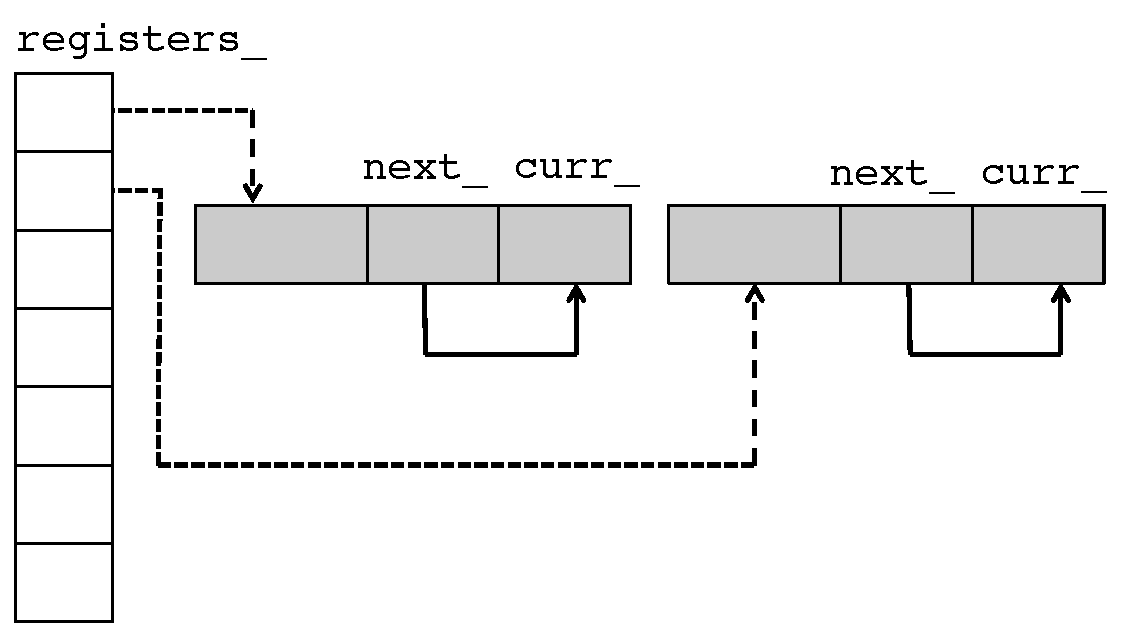
\includegraphics[clip,width=\linewidth-30pt]{simple_reg}
 \caption{シンプルな実装による reg クラスのインスタンスの処理の様子}
 \label{fig:regs}
\end{figure}

\figref{fig:regs} はシンプルな実装による reg クラスのインスタンスの処理の様子である.\figref{src:class_singleton}
の 44 行から 46 行の処理を表している.reg クラスのインスタンスが灰色に塗られており,左からクラスのメタデータ,next\_, curr\_
を表している.左側の大きな枠が\figref{src:class_singleton} の 18 行の \verb`std::vector` 型の registers\_ である.
実線矢印は代入を表し.点線矢印はポインタ参照を表す.

ArchHDL ではノン・ブロッキング代入をシミュレーションするために registers\_ の値を上から順に辿り,reg クラスの各インスタンスのポインタを取得する.そして reg クラスの全インスタンスの reg::Update() メソッドを呼ぶ.

\ref{sss:no_set} 節で述べたデータ変更の有無による条件分岐の除去を行うと
reg::Update() メソッド内で行なっている reg
クラスのインスタンスの curr\_ に next\_ の値を代入する処理は毎サイクル全
reg クラスのインスタンスで実行されることになる.

この代入する処理と reg::Update() メソッドの関数呼び出しの 2
つのオーバーヘッドが ArchHDL の高速化を妨げている.

\begin{figure}[t]
 \centering
 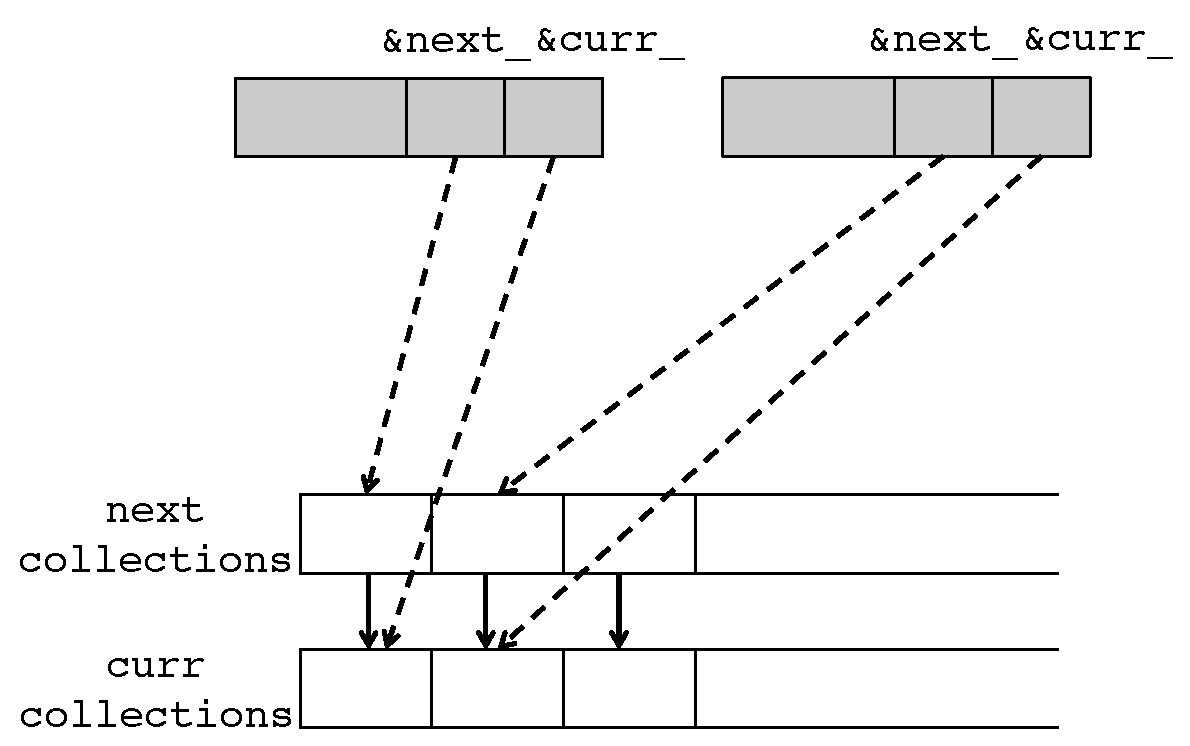
\includegraphics[clip,width=\linewidth-30pt]{mem_copy}
 \caption{値を配列として格納しポインタ参照を削減するように変更した reg クラスのインスタンスの処理の様子}
 \label{fig:mem_copy}
\end{figure}

\figref{fig:mem_copy} に提案手法を示す.\figref{fig:mem_copy} では値を配列として格納しポインタ参照を削減するように変更した reg クラスのインスタンスの処理の様子を表す.reg クラスのインスタンスが灰色に塗られており,左からクラスのメタデータ,\&next\_, \&curr\_ を表している.\&next\_, \&curr\_ は next\_, curr\_ のポインタである.
下の枠が next\_, curr\_ の値をまとめた配列であり,ここでは next collections, curr collections と呼ぶ.
実線矢印は代入を表し.点線矢印はポインタ参照を表す.

このように,全 reg クラスのインスタンスは現在の値と次サイクルの値の実体は持たず,ポインタを保持するように変更している.

次サイクルに移る前に行われる curr\_ に next\_ の値を代入する処理は \figref{fig:regs} で示すシンプルな実装では registers\_ から reg クラスのインスタンスが存在するアドレスを調べる必要がある.
しかし値を配列として格納しポインタ参照を削減すると \figref{fig:mem_copy} に示すように単純な代入となる.これにより代入する処理が高速になることが期待される.

これにより今まで飛び飛びのアドレスに格納されていた next\_ と curr\_ のメモリ配置がまとまるので高速になることが期待される.
また reg::Update() の関数呼び出しが不要となり,関数呼び出しのオーバーヘッドもなくなる.

提案手法の実装について述べる.next collections, curr collections として 2 つの十分大きな \verb/unsigned int/ 型の配列を用意する.記述された型に応じて,reg クラスのコンストラクタが next\_, curr\_ それぞれの領域を next collections, curr collections に確保する.
参照の高速化のために 4 バイトの倍数として領域を確保する.
確保された next\_ と curr\_ のアドレスを取得し,インスタンス内の \&next\_, \&curr\_ がそれを保持する.
これまで reg クラスの全インスタンスの reg::Update() メソッドを呼び出していたところを next\_ collections から curr\_ collections の値コピーに変更する.


\if0
\subsubsection{ダブルバッファリング}

これまでの実装では \ref{ss:implementation} 章で述べたように reg
クラスのインスタンスの次サイクルの値が次サイクルに移る前に reg
クラスのインスタンスの現在の値に代入される.
そこで偶数回目の実行と奇数回目の実行で次サイクルの値と現在の値を格納している変数を
を入れ替えれば(ダブルバッファリング)代入が減ることが期待できる.

\begin{figure}[t]
 \begin{center}
  \setlength{\unitlength}{1truemm} %picture環境の単位が1mmになる
\begin{picture}(60,13)(0,-3)
 \put(10,0){\framebox(10,10){\texttt{next\_}}}
 \put(40,0){\framebox(10,10){\texttt{curr\_}}}
 \put(0,5){\vector(1,0){8}}
 \put(0,7){\texttt{write}}
 \put(22,7){\texttt{every cycle}}
 \put(22,5){\vector(1,0){16}}
 \put(22,2){\texttt{\phantom{sss}write}}
 \put(52,5){\vector(1,0){8}}
 \put(52.5,7){\texttt{read}}
\end{picture}
 \end{center}
 \caption{reg クラスのインスタンスの変数保持の処理の様子}
 \label{fig:reg_curr_next}
\end{figure}

\begin{figure}[t]
 \begin{center}
  \setlength{\unitlength}{1truemm} %picture環境の単位が1mmになる
\begin{picture}(85,33)(0,-3)
 \put(35,20){\framebox(10,10){}}
 \put(55,20){\framebox(10,10){}}
 \put(35,0){\framebox(10,10){}}
 \put(55,0){\framebox(10,10){}}
 \put(25,25){\vector(1,0){8}}
 \put(25,27){\texttt{write}}
 \put(67,25){\vector(1,0){8}}
 \put(67.5,27){\texttt{read}}
 % bottom
 \put(33,5){\vector(-1,0){8}}
 \put(25.5,7){\texttt{read}}
 \put(75,5){\vector(-1,0){8}}
 \put(67.5,7){\texttt{write}}
 % round arrow
 \qbezier(2.5,8)(0,15)(2.5,22)
 \put(2.5,22){\vector(1,2){1}}
 \put(2.5,8){\vector(1,-2){1}}
 % cycle
 \put(5,23){\texttt{odd cycle}}
 \put(5,6){\texttt{even cycle}}
\end{picture}
 \end{center}
 \caption{ダブルバッファリングの処理の様子}
 \label{fig:double_buffer}
\end{figure}

\figref{fig:reg_curr_next} はこれまでの ArchHDL の reg
クラスのインスタンスの値の保持のイメージである.読み込み用と書き込み用の変数をそれぞれ保持している.読み込み用が現在の値であり,書き込み用が次サイクルの値である,次サイクルに移る前に書き込み用の値が読み込み用の変数に書き込まれる.

\figref{fig:double_buffer}
はダブルバッファリングのイメージである.奇数回目のサイクルと偶数回目のサイクルで読み込み用と書き込み用の変数を入れ替える.これにより奇数回目のサイクルで書き込み用であった変数には値が書き込まれているので次サイクルの偶数回目のサイクルで読み込み用として使用出来る.これを繰り返すことで,次サイクルに移る前に行われる代入処理を無くせる.

しかし今回の手法では reg
クラスのインスタンスへ値の書き込みが行われなかった場合に reg
クラスのインスタンスのその時の書き込み用の値に更新が入らない.次サイクルではその書き込み用の値がそのまま現在の値として使用されるので古い値が使われてしまう.そのため単純に入れ替えるだけの実装では誤ったシミュレーションを行なってしまう.

また今回の手法はサイクルの回数で依存関係が発生するので \ref{ss:parallel}
節で述べる並列化ができない.

よってライブラリの実装として導入するのは困難であるが,reg
クラスのインスタンスへ常に書き込みが行われるカウンター回路で試したところ効果があった(具体的な数字).常に
reg
クラスのインスタンスに書き込みが行われるハードウェアシミュレーションを逐次処理で行いたい場合には高い効果が期待できる.

以上の理由から本論文ではダブルバッファリングによる評価は行わない.

\fi

\subsection{並列化による高速化} \label{ss:parallel}

これまで逐次実行による高速化を考えてきたが,本節では並列化による高速化について考える.

\figref{src:class_singleton} の 40 行〜 47 行に示すように
毎サイクル,Module クラスと reg クラスの全インスタンスの Module::Always() メソッドと reg::Update() メソッドが呼び出されている.

\figref{src:class_singleton} の41行〜43行で実行される Module::Always() メソッドはユーザが自由に記述できる.
そのため各 Module クラスのインスタンスで独立に Module::Always() メソッドが実行できる保証はない.しかしここでは独立に実行できると仮定する.
このため\figref{src:class_singleton} の41行〜43行に示している Module::Always() メソッドの実行は並列化ができる.
独立に実行できる条件は今後の研究課題とする.

\figref{src:class_singleton} の 44 行〜 46 行で行われるレジスタの更新は\figref{fig:regs} の実線で表されている.各インスタンスで独立に行えるので並列化が可能である.

提案手法について述べる.以上のことから\figref{src:class_singleton} の41行〜47行に示している
Module クラスと reg クラスの全インスタンスの Module::Always() メソッドと reg::Update() メソッドの実行は並列化が可能である.
よってこの部分を並列化する.並列化には OpenMP~\cite{openmp} を用いる.

\begin{figure}[t]
 \lstinputlisting[language=c++]{src/exec_openmp.cc}
 \caption{Exec メソッド内の for 文を OpenMP で並列化したプログラム}
 \label{src:exec_openmp}
\end{figure}

\figref{src:exec_openmp} は\figref{src:class_singleton} の 40 行〜 47 行を 8 スレッドで並列化されるように OpenMP 指示文を与えたソースコードである.
4 行目と 8 行目は for 文の実行を並列化する OpenMP 指示文である.
2 行目は並列化を何スレッドで行うかを与えている.今回は 8 をスレッド数に指定している.この数字は環境によって変わる.

一般に並列化を行う場合は各スレッドに対して均等に負荷を与えることが重要である.
for 文の負荷を分散するスケジュール方法として静的に決定する static と,動的に決定する dynamic など複数存在する.
一般にスケジュール方法に dynamic を指定した場合,オーバーヘッドが大きい.
よって各モジュールと各レジスタで実行時間が大幅に変わらない限り,static を指定した方が効率が良いと考えられる.
実際に dynamic を指定すると遅くなることが確認されている.

他にも OpenMP にはオプションとしてチャンクサイズ(割り当てサイズ)を指定できる.
スケジュール方法を static にし,チャンクサイズを指定しなければ,チャンクサイズはループの反復数をスレッド数で割った商とほぼ同じ値になる.
チャンクサイズを指定するとデフォルトよりも遅くなることが確認されている.

よって今回の評価はスケジュール方法が static でチャンクサイズは指定しないというデフォルトの設定で行う.
